\documentclass[../main.tex]{subfiles}

\begin{document}
Im ersten Teil dieser Arbeit soll eine rein seriellen Implementierung eines Convolutional Neural Network erstellt werden. Als Vorlage dient ein ein von Google veröffentlichtes Python-Skript, das die Bibliothek TensorFlow verwendet. Ziel dieser ersten Implementierung ist nicht, eine produktiv anwendbare Software zu erstellen, sondern eine in C++ geschriebene Vorlage für die später zu erstellenden optimierten Implementierungen zu schaffen. 
\section{Tensorflow}
TensorFlow ist eine von Google entwickelte und veröffentlichte Bibliothek für hochperformante numerische Berechnungen. Anwendung findet TensorFlow unter anderem in den Bereichen Machine Learning und Deep Learning. Dazu gehört auch die Erkennung handgeschriebener Ziffern mithilfe eines Convolutional Neural Network. APIs zur Interaktion mit TensorFlow existieren in mehreren Programmiersprachen, am weitesten verbreitet ist allerdings Python. Die eigentlichen Berechnungen werden allerdings von einer vorkompilierten Bibliothek durchgeführt, um Overhead von interpretierten Sprachen oder mangelhafter Compileroptimierung zu vermeiden. (vgl. \cite{tensorflowTutorial2})
\section{Netzaufbau}
Der für die serielle Implementierung verwendete Netzaufbau wird von einem Python-Skript übernommen, das Google mit der offiziellen Dokumentation von Tensorflow veröffentlicht hat. (vgl. \cite{tensorflowTutorial})
\begin{figure}
    \centering 
       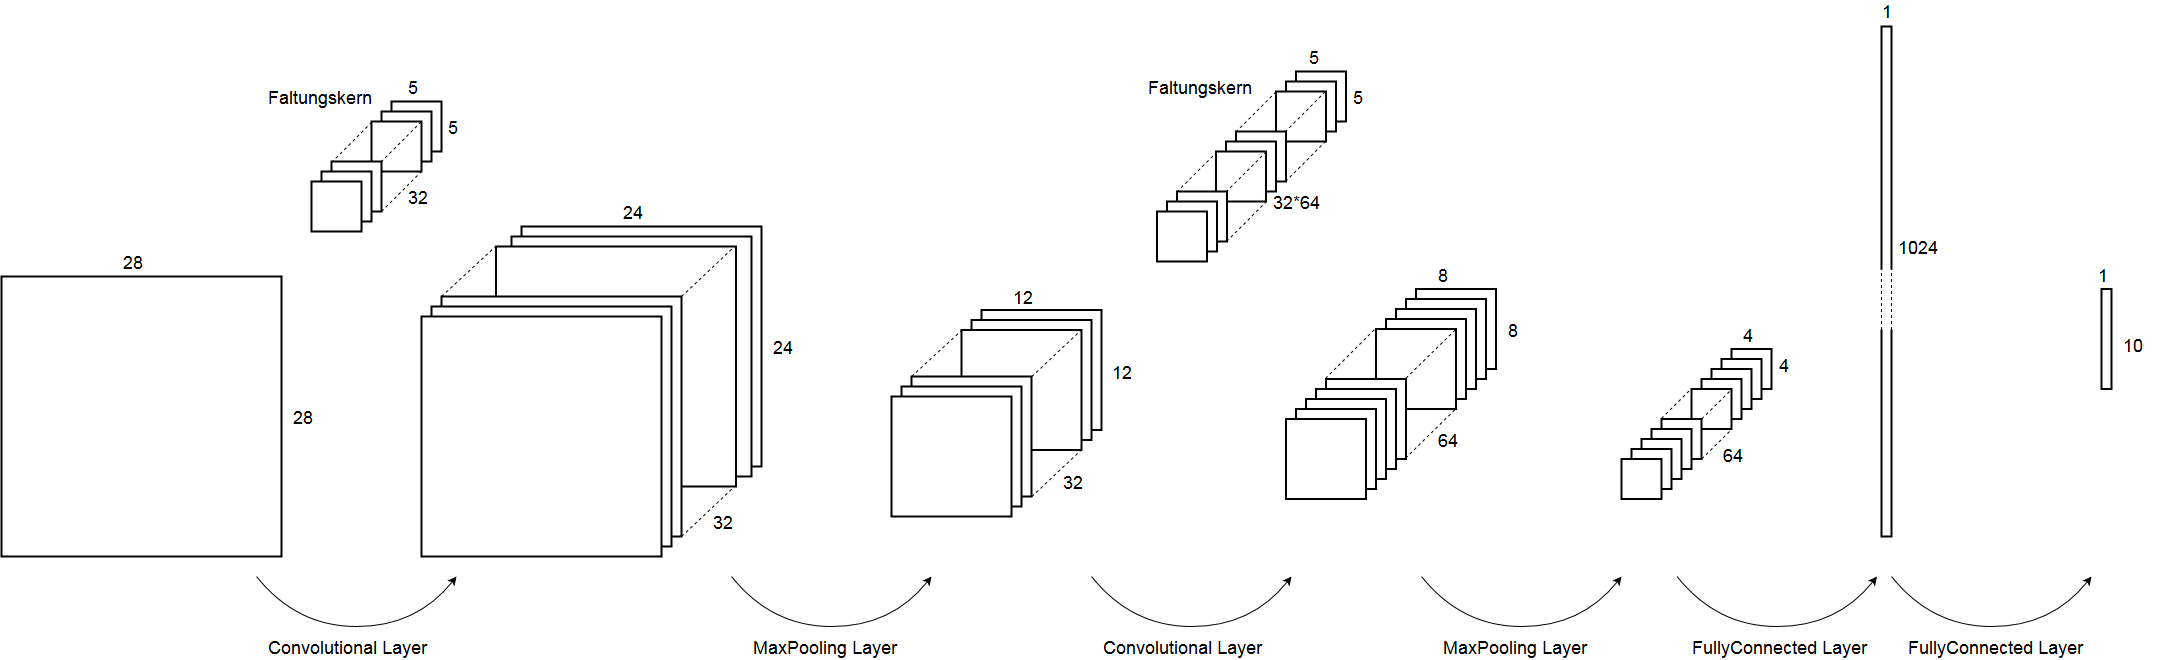
\includegraphics[width=\textwidth]{../images/Benz/Aufbau_Netzwerk.png} 
    \caption {Schematische Darstellung des Netzaufbaus in der seriellen Implementierung} 
    \label{pic:AufbauNetzwerkSerial} 
\end{figure} 
Die Abfolge der verwendeten Schichten, sowie einige ihrer Eigenschaften sind in Abbildung \ref{pic:AufbauNetzwerkSerial} schematisch dargestellt. Wie darin zu sehen ist, besteht das Netz aus 6 Schichten. Zwei Paare aus je einem Convolutional Layer und einem Max Pooling Layer werden von zwei Fullyconnected Layern gefolgt. Für die in der Vorlage verwendeten Filtergrößen und Featurezahlen ist bekannt, dass sie zu einer Testgenauigkeit von etwa 98\,\% führen sollten. (vgl. \cite{tensorflowTutorial}) Aufgrund einiger Abweichungen von der Vorlage kann die Erwartungshaltung an die Genauigkeit allerdings nicht ohne Vorbehalte auf den Netzaufbau in dieser Arbeit übertragen werden. Grund dafür sind einige Abweichungen des Aufbaus von der Vorlage. Als Aktivierungsfunktion wird in dieser Arbeit sigmoid verwendet. Außerdem wird beim Trainieren in der Vorlage eine Technik namens Dropout Regularization eingesetzt. Diese Technik steigert die erreichbare Testgenauigkeit, indem sie einen störenden Effekt namens Overfitting vermindert. (vgl. \cite{neuralNetworksAndDeepLearning})
\section{Systembeschreibung}
Das Programm der seriellen Implementierung muss folgende Aufgaben erfüllen: 
\begin{description}
\item{Trainings- und Testdaten:} Die zu verarbeitenden Bilder müssen gemeinsam mit den Labels zur Laufzeit von der Festplatte eingelesen werden. 
\item{Netzwerkmodell:} Das Programm muss ein internes Modell des Netzwerks besitzen, durch das festgelegt wird, wie die Bilder zu verarbeiten sind. Außerdem sind im Netzwerkmodell die veränderlichen Gewichte angesiedelt. 
\item{Training:} Beim Training müssen die Eingabedaten das Netzwerk zunächst vorwärts durchlaufen. Anschließend wird zur Fehlerberechnung eine Backpropagation durchgeführt und die Gewichtsanpassung mittels Gradient Descent vorgenommen. 
Der Trainingsprozess wird für alle Trainingsdaten mehrfach wiederholt. Das einmalige Trainieren mit jedem Bild der Trainingsdaten wird als Epoche bezeichnet. 
\item{Test:} Zum Testen werden von den Trainingsbildern verschiedene Eingaben verwendet. Diese durchlaufen das Netzwerk zunächst in Vorwärtsrichtung. Anschließend werden die Ergebnisse mit den Labels verglichen. Die Abweichung des Ergebnisses vom erwarteten Wert gemäß des labels ist ausschlaggebend für die Kosten. Die Genauigkeit entspricht dem Anteil der Testfälle, für die die Eingabe gemäß der Erwartungen basierend auf dem Wert des Labels richtig klassifiziert wurde. 
\end{description}
Gemäß dieser Erwartungen wird zunächst eine grobe Architektur entworfen, die in Abbildung \ref{pic:cnn_serial_classes} durch ein Klassendiagramm visualisiert wird. 
\begin{figure}
    \centering 
       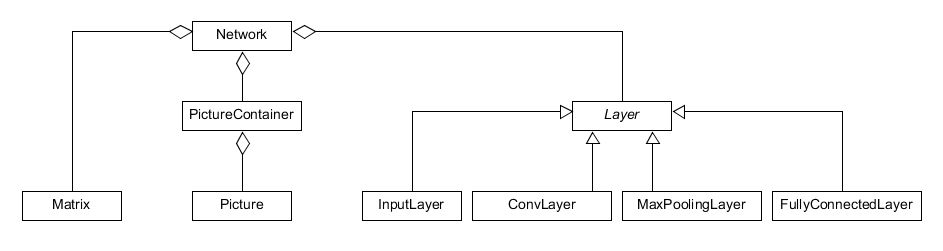
\includegraphics[width=\textwidth]{../images/Schmidt/CNN_Serial_Classes.jpg} 
    \caption {Klassendiagramm der seriellen Implementierung} 
    \label{pic:cnn_serial_classes} 
\end{figure} 
Die im Diagramm \ref{pic:cnn_serial_classes} dargestellten Klassen sind gemäß ihrer Aufgabenbereiche voneinander abgegrenzt. Eine nähere Erläuterung der Einsatzzwecke dieser Klassen erfolgt an dieser Stelle nach dem Bottom-Up-Ansatz: 
\begin{description}
\item{Matrix:} Diese Klasse repräsentiert eine Matrix von beliebiger Größe. Bei der Erstellung wird die Größe der Matrix an den Konstruktor übergeben, woraufhin dieser einen entsprechend großen Speicherbereich alloziert. Die Klasse stellt Operationen zur Verfügung, mit denen Matrizen addiert, multipliziert und skaliert werden können. Außerdem können sie mit zufälligen oder vorgegebenen Werten gefüllt werden. 
\item{Picture:} Jede Instanz der Klasse Picture repräsentiert jeweils ein Eingabebild gemeinsam mit dem einem Vektor, der dem Wunschwert für die Ausgabe entspricht. Die Ein- und Ausgabedaten werden jeweils als Array innerhalb des Objekts gespeichert. Es lassen sich Matrix-Objekte erzeugen, die auf den Speicherbereich der Arrays innerhalb eines Picture-Objekts verweisen. Auf diese Weise können die im Picture enthaltenen Informationen leicht zur Weiterverarbeitung in Layern konvertiert werden. 
\item{PictureContainer:} Der PictureContainer repräsentiert eine Ansammlung von Picture-Objekten. Es ist vorgesehen, dass sowohl für die Trainingsdaten, als auch für die Testdaten jeweils eine Instanz dieser Klasse existiert. Ein PictureContainer beinhaltet zudem eine Funktion, durch deren mehrfachen Aufruf über alle enthaltenen Bilder iteriert werden kann. Um den Speicherbedarf zu begrenzen, hält ein PictureContainer normalerweise 1000 Picture-Objekte im Arbeitsspeicher. Wenn über alle Bilder iteriert wurde, wird automatisch eine Datei von der Festplatte ausgelesen, die weitere Ein- und Ausgabedaten zum erzeugen neuer Picture-Objekte  bereitstellt. 
\item{Layer:} Diese abstrakte Klasse dient als Basis für alle Layertypen. Darin enthalten sind Informationen, die das Verhalten und die Eigenschaften einer Schicht beschreiben. Die von Layer abgeleiteten Klassen können zusätzliche Eigenschaften enthalten, die für den jeweiligen Layertyp spezifisch sind. Veränderliche Gewichte und Aktivierungen sind in den Objekten dieser Klasse nicht enthalten. 
\item{Network:} Dies ist die zentrale Klasse des seriellen Programms. Zur Laufzeit existiert genau ein Objekt dieser Klasse. Dieses verwaltet die PictureContainer mit den Trainings- und Testdaten, eine Liste von Layer-Objekten zur Definition des Netzwerkmodells und eine mehrere Listen von Matrix-Objekten zur Speicherung aller veränderlichen Gewichte, Aktivierungen und Fehlergrößen. In dieser Klasse sind auch die Methoden zur Forward- und Backpropagation, zur Gewichtsanpassung und zum Trainingsablauf definiert. 
\item{main:} Die Main-Funktion erzeugt ein Objekt der Klasse Network und initialisiert die Liste der Layer, um das Netzwerkmodell festzulegen. Anschließend ruft es die Trainings- und Testmethoden des Netzwerks auf. 
\end{description}
\section{Beschreibung der Problematik einer seriellen Implementierung}
Prinzipiell sollte das oben beschriebene Programm bei fehlerfreier Implementierung bereits in der Lage sein, anhand der Trainingsdaten das Klassifizieren von handgeschriebenen Ziffern automatisiert zu erlernen und dabei eine Genauigkeit im Bereich von 90\,\% bis 95\,\% zu erreichen. Dies lässt sich allerdings nicht in annehmbarer Zeit überprüfen. Aufgrund dessen, dass es rein seriell arbeitet und nicht optimiert ist, würde es sehr lange dauern, bis eine nennenswerte Steigerung der Genauigkeit erkennbar ist. 
\end{document}